\section{Main Window}
\label{sec:ui_main_window} 

When the application is started for the first time, the main window is shown as follows. 

\begin{figure}[H]
  \centering
  \hspace*{-2.5cm}
    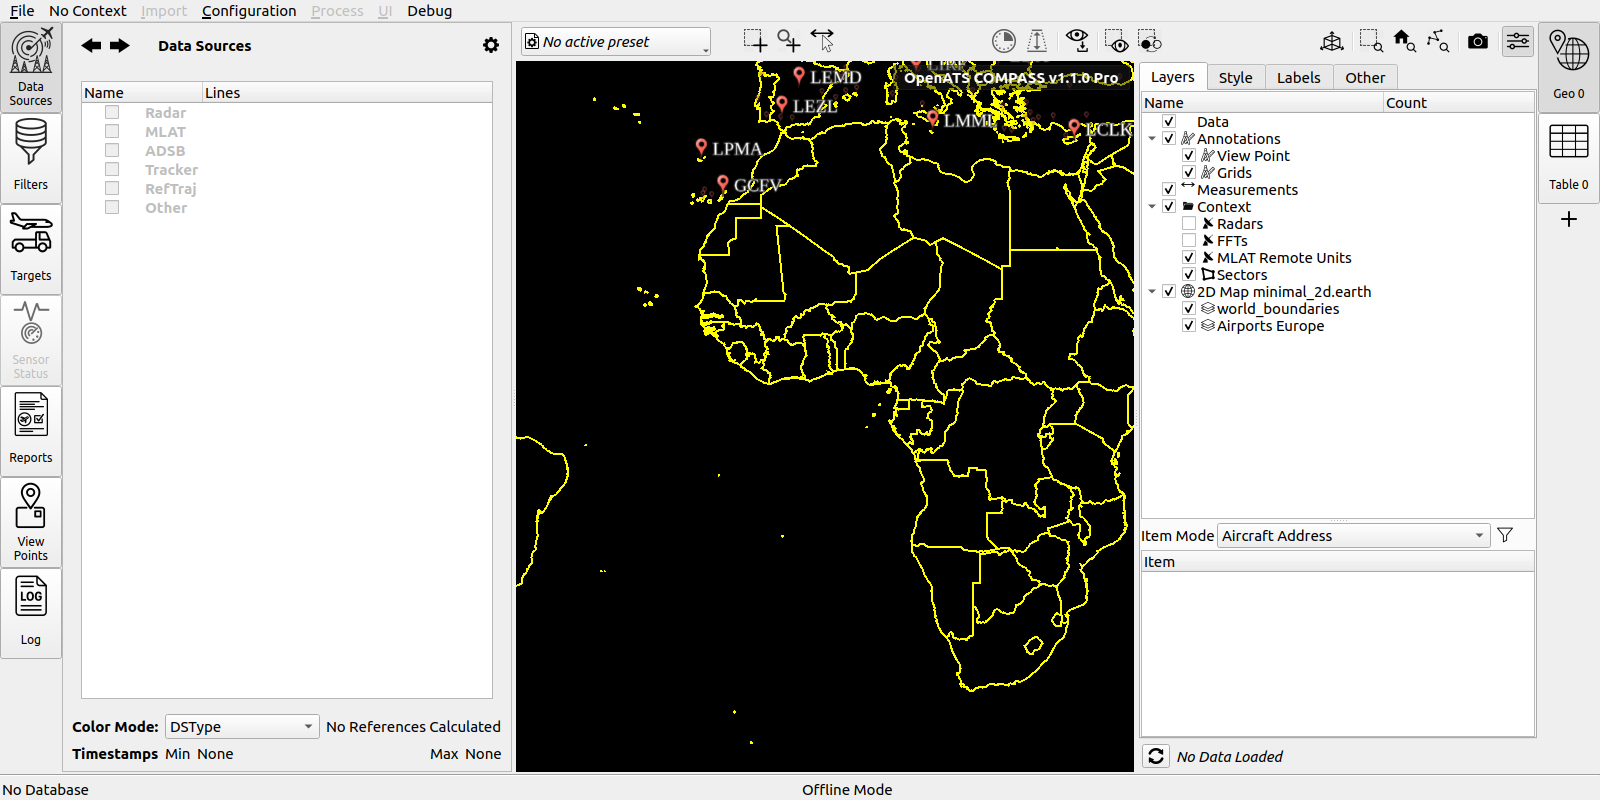
\includegraphics[width=19cm,frame]{figures/main_window.png}
  \caption{Main Window}
\end{figure}

Below the \nameref{sec:ui_main_menu_bar}, the main window has two parts:
\begin{itemize}
 \item \nameref{sec:ui_flight_deck}: On the left side, the tools to select, filter and inspect data
 \item \nameref{sec:ui_view_deck}: On the right side, the Views that show the loaded data
\end{itemize}
\  \\

Both decks work the same way. Each deck has an icon bar at the window edge. A click on an icon shows the tool or the View. A deck can be collapsed to its icon bar, so the other deck gets the full width. \\

\begin{figure}[H]
  \centering
  \hspace*{-2.5cm}
    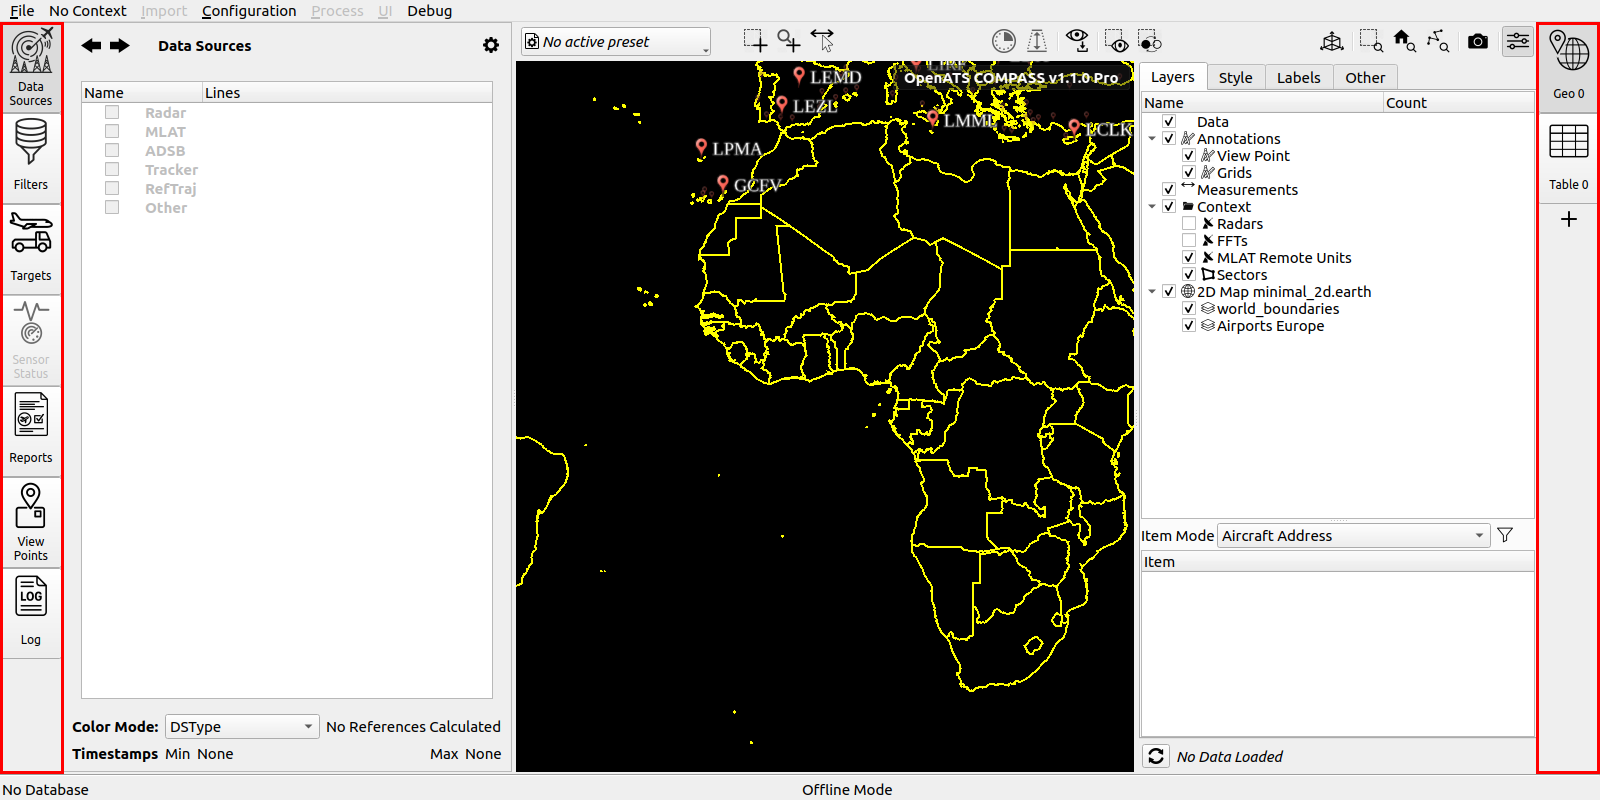
\includegraphics[width=19cm,frame]{figures/ui_decks.png}
  \caption{Main Window: Flight Deck icon bar (left) and View Deck icon bar (right)}
\end{figure}

In the simplest use case, the \nameref{sec:ui_main_menu_bar} allows opening or creating a database and importing data (using a given Data Context).
After this step, data of interest can be chosen using the tools of the Flight Deck,
and loaded from the database using the 'Load' button of the \nameref{sec:ui_main_status_bar}.
The loaded data is then shown in Views located either in the View Deck of the main window, or in other windows. \\

The values set in the 'Data Sources' and 'Filter' tools of the Flight Deck define the dataset loaded from the database into memory (RAM). 
Only the data required by the application is loaded into memory. \\

Only one dataset can exist at a time. At the beginning of a loading process, the old dataset is cleared, and a new one is filled sequentially from the database. 
This single dataset is then distributed to all existing views. \\

When new Views are added, or Views require additional data, a manual reload has to be performed by the user. \\

To close the application either the 'File' menu or the close button in the main window's decoration bar can be used. \\

Please \textbf{note} that using the close button in windows other than the main window only closes the respective window and its Views, but not the application.

Please \textbf{note} that depending on the application status some parts of the UI are inaccessible, e.g. are only available when a database was opened.

\subsection{Main Menubar}
\label{sec:ui_main_menu_bar}

At the top of the Main Window exists the Main Menubar, which contains the Main Menu and allows access to the following sub-menus: 

\begin{itemize}
 \item \nameref{sec:ui_overview_file_menu}: Open/close a database, quit application
 \item \nameref{sec:ui_overview_context_menu}: Manage the active Data Context
 \item \nameref{sec:ui_overview_import_menu}: Import ASTERIX, NMEA data
 \item \nameref{sec:ui_overview_config_menu}: Configure data sources, sectors, manage licenses
 \item \nameref{sec:ui_overview_process_menu}: Various processing tasks for imported data
 \item \nameref{sec:ui_overview_ui_menu}: Reset Views
\end{itemize} 
\  \\

A common workflow is to open or create a database using the 'File' menu. Before any data can be imported, an active Data Context must contain the data sources of the recording (see \nameref{sec:configure_data_context}). If new data is to be imported, this can be done using the 'Import' menu. After all data was imported, the 'Process' menu can be used to post-process the data in various ways. \\

For a more detailed description of the Main Menu's contents refer to section \nameref{sec:main_menu}.

\subsection{Flight Deck} 
\label{sec:ui_flight_deck}

\begin{figure}[H]
  \centering
  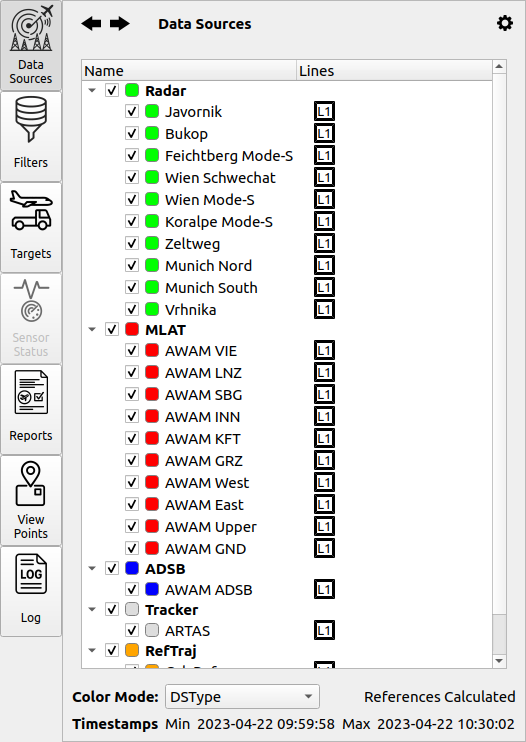
\includegraphics[width=12cm, frame]{figures/ui_flight_deck.png}
  \caption{Opened Flight Deck}
\end{figure}

The Flight Deck is a special tool bar located on the left side of the main window, and allows for quick access to 
frequently used functionality. It can be quickly expanded and collapsed, and its tools can be viewed alongside a View,
making working in a single monitor setup more comfortable. \\

The following tools exist in the Flight Deck:

\begin{table}[H]
  \center
  \begin{tabular}{ | l | l | l | }
    \hline
    \textbf{Tool} & \textbf{Hotkey} & \textbf{Description} \\ \hline
    \nameref{sec:data_sources} & 1 & Select which data sources and lines should be loaded \\ \hline
    \nameref{sec:filters} & 2 & Filter which data should be loaded \\ \hline
    \nameref{sec:targets} & 3 & Allows inspection of unique targets after reference reconstruction \\ \hline
    \nameref{sec:sensor_status} & 4 & Allows inspection of sensor states in Live Mode \\ \hline
    \nameref{sec:reports} & 5 & Allows inspection of previously generated Reports (e.g. Evaluation Reports) \\ \hline
    \nameref{sec:view_points} & 6 & Show/edit specific cases saved as View Points \\ \hline
    \nameref{sec:task_log} & 7 & Persistent event log, showing important events occurring during COMPASS usage \\ \hline
  \end{tabular}
  \caption{Flight Deck: Available tools}
  \label{table:ui_flight_deck_tools}
\end{table}

% \begin{itemize}
%  \item \nameref{sec:ui_data_sources}: Select which data sources and lines should be loaded
%  \item \nameref{sec:ui_filters}: Filter which data should be loaded
%  \item \nameref{sec:ui_targets}: Allows inspection of unique targets after reference reconstruction
%  \item \nameref{sec:reports}: Allows inspection of previously generated Reports (e.g. Evaluation Reports) %adapting/defining requirement-based standards and compliance assessment of said standards
%  \item \nameref{sec:view_points}: Show/edit specific cases saved as View Points
%  \item \nameref{sec:log}: Persistent event log, showing important events occurring during COMPASS usage (information, warnings, errors)
% \end{itemize}
% \  \\

The individual tools will be described in more detail in Chapter \nameref{chap:flight_deck}. \\

A tool can be selected by clicking its respective icon. This will also show the Flight Deck again if it was previously closed.
Clicking the icon of a selected tool again will collapse the Flight Deck to its icon bar, and the \nameref{sec:ui_view_deck} gets the full width.
If the View Deck was collapsed before, it opens again with its last View. Switching between tools can also be achieved by pressing
the number keys on the keyboard. Pressing the respective number key will show the tool (and possibly show the Flight Deck again),
pressing it again will collapse the Flight Deck. Table \ref{table:ui_flight_deck_tools} lists the assigned number hotkeys. \\

The width of the Flight Deck is set per tool, in percent of the main window width next to the icon bar:

\begin{itemize}
\item Drag the separator between the Flight Deck and the View Deck: the width changes in steps of 10 percent
\item 'Decrease Width' \includegraphics[width=0.5cm,frame]{../../data/icons/arrow_to_left.png} and 'Increase Width' \includegraphics[width=0.5cm,frame]{../../data/icons/arrow_to_right.png} buttons at the top of each tool, or the keys '-' and '+': change the width by 10 percent
\item The width is between 10 and 70 percent, also limited by the minimum widths of the tool and the Views
\item Each tool keeps its own width, also after a restart of the application
\end{itemize}
\ \\

When selecting a tool, the tools content will be shown with a decoration bar on top. The bar will show the selected tool's name 
and various action buttons for configuring the tool.

\begin{table}[H]
  \center
  \begin{tabular}{ | l | l | l | l |}
    \hline
    \textbf{Icon} & \textbf{Shortcut} &\textbf{Text} & \textbf{Description} \\ \hline
    \includegraphics[width=0.5cm,frame]{../../data/icons/arrow_to_left.png} & - & Decrease Width & Decrease Flight Deck width for the selected tool \\ \hline
    \includegraphics[width=0.5cm,frame]{../../data/icons/arrow_to_right.png} & + & Increase Width & Increase Flight Deck width for the selected tool \\ \hline
    \includegraphics[width=0.5cm,frame]{../../data/icons/edit.png} & & & Open the selected tool's configuration menu \\ \hline
  \end{tabular}
  \caption{Toolbar: Available actions}
\end{table}

\paragraph{Tool Configuration Menu} Pressing the \includegraphics[width=0.5cm,frame]{../../data/icons/edit.png} button will
open a menu with tool-specific configuration options.

\begin{figure}[H]
  \centering
  \hspace*{-0.5cm}
  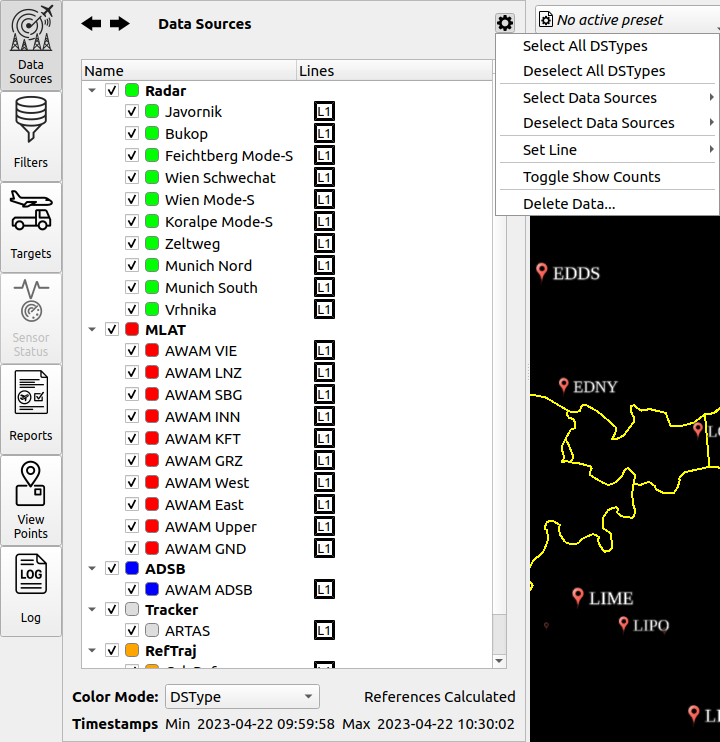
\includegraphics[width=15cm,frame]{figures/ui_flight_deck_config.png}
  \caption{Flight Deck: Tool configuration menu}
\end{figure}

\subsection{View Deck}
\label{sec:ui_view_deck}

The \textbf{View Deck} holds the Views of a window. It works the same way as the Flight Deck. Its icon bar is at the right edge of the window. \\

\begin{itemize}
 \item View icons: Each View has an icon in the icon bar
 \begin{itemize}
  \item The icon shows the type of the View
  \item The short name below the icon gives the type and the number of the View, e.g. 'Geo 0' or 'Table 0'
  \item The tooltip shows the full name of the View
 \end{itemize}
 \item Show a View: Click its icon
 \item Collapse the View Deck: Click the icon of the shown View again
 \begin{itemize}
  \item The View Deck collapses to its icon bar, and the Flight Deck gets the full width
  \item If the Flight Deck was collapsed before, it opens again with its last tool
  \item A click on any View icon opens the View Deck again
 \end{itemize}
 \item Add a View: Click the \includegraphics[width=0.5cm,frame]{../../data/icons/crosshair_fat.png} button at the end of the icon bar
 \begin{itemize}
  \item 'Add Here': Adds the View to the View Deck of this window
  \item 'Add In New Window': Adds the View to a new window
 \end{itemize}
 \item Close a View: Move the mouse over its icon and click the \includegraphics[width=0.5cm,frame]{../../data/icons/delete.png} button ('Close View') at the top right of the icon
\end{itemize}
\  \\

The Flight Deck and the View Deck are never collapsed at the same time. \\

Other COMPASS windows also have a View Deck. These windows have no Flight Deck, so a click on the icon of the shown View does not collapse the View Deck. \\

See section \nameref{sec:ui_views} for more details about Views.

\subsection{Main Statusbar}
\label{sec:ui_main_status_bar}

The Main Statusbar at the bottom shows general information and contains the 'Load' button used to trigger a loading process (only visible when a database was opened). \\

The following information is shown:

\begin{itemize}
 \item Database indicator: Shows 'No Database' or currently opened database file name
 \item Application mode: 'Offline' or 'Live'
\end{itemize}
\  \\
